% !TeX root = RJwrapper.tex
\title{Blocking: An R Package for Blocking of Records for Record Linkage and Deduplication}


\author{by Maciej Beręsewicz and Adam Struzik}

\maketitle

\abstract{%
An abstract of less than 250 words.
}

\section{Introduction}\label{introduction}

Interactive data graphics provides plots that allow users to interact them. One of the most basic types of interaction is through tooltips, where users are provided additional information about elements in the plot by moving the cursor over the plot.

This paper will first review some R packages on interactive graphics and their tooltip implementations. A new package \CRANpkg{ToOoOlTiPs} that provides customized tooltips for plot, is introduced. Some example plots will then be given to showcase how these tooltips help users to better read the graphics.

\section{Background}\label{background}

Some packages on interactive graphics include \CRANpkg{plotly} \citep{plotly} that interfaces with Javascript for web-based interactive graphics, \CRANpkg{crosstalk} \citep{crosstalk} that specializes cross-linking elements across individual graphics. The recent R Journal paper \CRANpkg{tsibbletalk} \citep{RJ-2021-050} provides a good example of including interactive graphics into an article for the journal. It has both a set of linked plots, and also an animated gif example, illustrating linking between time series plots and feature summaries.

\section{\texorpdfstring{Blocking of records using \texttt{blocking} function}{Blocking of records using blocking function}}\label{blocking-of-records-using-blocking-function}

\section{Integration with existing packages}\label{integration-with-existing-packages}

\section{Case study}\label{case-study}

\subsection{Record linkage example}\label{record-linkage-example}

Let us first load the required packages.

\begin{verbatim}
library(blocking)
library(data.table)
\end{verbatim}

We demonstrate the use of \texttt{blocking} function for record linkage on the \texttt{foreigners} dataset included in the package. This fictional representation of the foreign population in Poland was generated based on publicly available information, preserving the distributions from administrative registers. It contains 110,000 rows with 100,000 entities. Each row represents one record, with the following columns:

\begin{itemize}
\tightlist
\item
  \texttt{fname} -- first name,
\item
  \texttt{sname} -- second name,
\item
  \texttt{surname} -- surname,
\item
  \texttt{date} -- date of birth,
\item
  \texttt{region} -- region (county),
\item
  \texttt{country} -- country,
\item
  \texttt{true\_id} -- person ID.
\end{itemize}

\begin{verbatim}
data(foreigners)
head(foreigners)
\end{verbatim}

\begin{verbatim}
#>     fname  sname    surname       date region country true_id
#>    <char> <char>     <char>     <char> <char>  <char>   <num>
#> 1:   emin            imanov 1998/02/05            031       0
#> 2: nurlan        suleymanli 2000/08/01            031       1
#> 3:   amio        maharrsmov 1939/03/08            031       2
#> 4:   amik        maharramof 1939/03/08            031       2
#> 5:   amil        maharramov 1993/03/08            031       2
#> 6:  gadir        jahangirov 1991/08/29            031       3
\end{verbatim}

We split the dataset into two separate files: one containing the first appearance of each entity in the \texttt{foreigners} dataset, and the other containing its subsequent appearances.

\begin{verbatim}
foreigners_1 <- foreigners[!duplicated(foreigners$true_id), ]
foreigners_2 <- foreigners[duplicated(foreigners$true_id), ]
\end{verbatim}

Now in both datasets we remove slashes from the \texttt{date} column and create a new string column that concatenates the information from all columns (excluding \texttt{true\_id}) in each row.

\begin{verbatim}
foreigners_1[, date := gsub("/", "", date)]
foreigners_1[, txt := paste0(fname, sname, surname, date, region, country)]
foreigners_2[, date := gsub("/", "", date)]
foreigners_2[, txt := paste0(fname, sname, surname, date, region, country)]
head(foreigners_1)
\end{verbatim}

\begin{verbatim}
#>     fname  sname    surname     date region country true_id
#>    <char> <char>     <char>   <char> <char>  <char>   <num>
#> 1:   emin            imanov 19980205            031       0
#> 2: nurlan        suleymanli 20000801            031       1
#> 3:   amio        maharrsmov 19390308            031       2
#> 4:  gadir        jahangirov 19910829            031       3
#> 5:   zaur         bayramova 19961006  01261     031       4
#> 6:   asif          mammadov 19970726            031       5
#>                              txt
#>                           <char>
#> 1:         eminimanov19980205031
#> 2:   nurlansuleymanli20000801031
#> 3:     amiomaharrsmov19390308031
#> 4:    gadirjahangirov19910829031
#> 5: zaurbayramova1996100601261031
#> 6:       asifmammadov19970726031
\end{verbatim}

\subsubsection{General use}\label{general-use}

We use the newly created columns in the \texttt{blocking} function, which relies on the default \CRANpkg{rnndescent} (Nearest Neighbor Descent) algorithm based on cosine distance. Additionally, we set \texttt{verbose\ =\ 1} to monitor progress. Note that a default parameter of the \texttt{blocking} function is \texttt{seed\ =\ 2023}, which sets the random seed.

\begin{verbatim}
result_reclin <- blocking(x = foreigners_1$txt,
                          y = foreigners_2$txt,
                          verbose = 1)
\end{verbatim}

\begin{verbatim}
#> ===== creating tokens =====
#> ===== starting search (nnd, x, y: 100000, 10000, t: 1232) =====
#> ===== creating graph =====
\end{verbatim}

Now we examine the results of record linkage.

\begin{itemize}
\tightlist
\item
  We have created 6,469 blocks.
\item
  The blocking process utilized 1,232 columns (2 character shingles).
\item
  We have 3,916 blocks of 2 elements, 1,604 blocks of 3 elements,\ldots, 2 blocks of 7 elements.
\end{itemize}

\begin{verbatim}
result_reclin
\end{verbatim}

\begin{verbatim}
#> ========================================================
#> Blocking based on the nnd method.
#> Number of blocks: 6469.
#> Number of columns used for blocking: 1232.
#> Reduction ratio: 0.9999.
#> ========================================================
#> Distribution of the size of the blocks:
#>    2    3    4    5    6    7 
#> 3916 1604  926   19    2    2
\end{verbatim}

Structure of the object is as follows:

\begin{itemize}
\tightlist
\item
  \texttt{result} -- a \texttt{data.table} with identifiers and block IDs,
\item
  \texttt{method} -- name of the ANN algorithm used,
\item
  \texttt{deduplication} -- whether deduplication was applied,
\item
  \texttt{representation} -- whether shingles or vectors were used,
\item
  \texttt{metrics} -- metrics for quality assessment (here \texttt{NULL}),
\item
  \texttt{confusion} -- confusion matrix (here \texttt{NULL}),
\item
  \texttt{colnames} -- column names used for the comparison,
\item
  \texttt{graph} -- an \CRANpkg{igraph} object, mainly for visualization (here \texttt{NULL}).
\end{itemize}

\begin{verbatim}
str(result_reclin, 1)
\end{verbatim}

\begin{verbatim}
#> List of 8
#>  $ result        :Classes 'data.table' and 'data.frame': 10000 obs. of  4 variables:
#>   ..- attr(*, ".internal.selfref")=<externalptr> 
#>  $ method        : chr "nnd"
#>  $ deduplication : logi FALSE
#>  $ representation: chr "shingles"
#>  $ metrics       : NULL
#>  $ confusion     : NULL
#>  $ colnames      : chr [1:1232] "0a" "0b" "0c" "0m" ...
#>  $ graph         : NULL
#>  - attr(*, "class")= chr "blocking"
\end{verbatim}

The resulting \texttt{data.table} has four columns:

\begin{itemize}
\tightlist
\item
  \texttt{x} -- reference dataset (i.e.~\texttt{foreigners\_1}) -- this may not contain all units of \texttt{foreigners\_1},
\item
  \texttt{y} -- query (each row of \texttt{foreigners\_2}) -- this may not contain all units of \texttt{foreigners\_2},
\item
  \texttt{block} -- block ID,
\item
  \texttt{dist} -- distance between objects.
\end{itemize}

\begin{verbatim}
head(result_reclin$result)
\end{verbatim}

\begin{verbatim}
#>        x     y block      dist
#>    <int> <int> <num>     <num>
#> 1:     3     1     1 0.2216882
#> 2:     3     2     1 0.2122737
#> 3:    21     3     2 0.1172652
#> 4:    57     4     3 0.1863238
#> 5:    57     5     3 0.1379310
#> 6:    61     6     4 0.2307692
\end{verbatim}

Let's examine the first pair. Obviously, there are typos in the \texttt{fname} and \texttt{surname}. Nevertheless, the pair is a match.

\begin{verbatim}
cbind(t(foreigners_1[3, 1:6]), t(foreigners_2[1, 1:6]))
\end{verbatim}

\begin{verbatim}
#>         [,1]         [,2]        
#> fname   "amio"       "amik"      
#> sname   ""           ""          
#> surname "maharrsmov" "maharramof"
#> date    "19390308"   "19390308"  
#> region  ""           ""          
#> country "031"        "031"
\end{verbatim}

Now we use the \texttt{true\_id} values to evaluate our approach.

\begin{verbatim}
matches <- merge(x = foreigners_1[, .(x = 1:.N, true_id)],
                 y = foreigners_2[, .(y = 1:.N, true_id)],
                 by = "true_id")
matches[, block := rleid(x)]
head(matches)
\end{verbatim}

\begin{verbatim}
#> Key: <true_id>
#>    true_id     x     y block
#>      <num> <int> <int> <int>
#> 1:       2     3     1     1
#> 2:       2     3     2     1
#> 3:      20    21     3     2
#> 4:      56    57     4     3
#> 5:      56    57     5     3
#> 6:      60    61     6     4
\end{verbatim}

We have 10,000 matched pairs. We use the \texttt{true\_blocks} parameter in the \texttt{blocking} function to specify the true block assignments. We obtain the quality metrics for the assessment of record linkage.

\begin{verbatim}
result_2_reclin <- blocking(x = foreigners_1$txt,
                            y = foreigners_2$txt,
                            verbose = 1,
                            true_blocks = matches[, .(x, y, block)])
\end{verbatim}

\begin{verbatim}
#> ===== creating tokens =====
#> ===== starting search (nnd, x, y: 100000, 10000, t: 1232) =====
#> ===== creating graph =====
\end{verbatim}

\begin{verbatim}
result_2_reclin
\end{verbatim}

\begin{verbatim}
#> ========================================================
#> Blocking based on the nnd method.
#> Number of blocks: 6469.
#> Number of columns used for blocking: 1232.
#> Reduction ratio: 0.9999.
#> ========================================================
#> Distribution of the size of the blocks:
#>    2    3    4    5    6    7 
#> 3916 1604  926   19    2    2 
#> ========================================================
#> Evaluation metrics (standard):
#>      recall   precision         fpr         fnr    accuracy specificity 
#>     96.7782     78.7000      0.0038      3.2218     99.9957     99.9962 
#>    f1_score 
#>     86.8079
\end{verbatim}

For example, our approach results in a 3.22\% false negative rate (FNR). To improve this, we can increase the \texttt{epsilon} parameter of the NND method from 0.1 to 0.5. To do so, we configure the \texttt{control\_ann} parameter in the \texttt{blocking} function using the \texttt{controls\_ann} and \texttt{control\_nnd} functions.

\begin{verbatim}
result_3_reclin <- blocking(x = foreigners_1$txt,
                            y = foreigners_2$txt,
                            verbose = 1,
                            true_blocks = matches[, .(x, y, block)],
                            control_ann = controls_ann(nnd = control_nnd(epsilon = 0.5)))
\end{verbatim}

\begin{verbatim}
#> ===== creating tokens =====
#> ===== starting search (nnd, x, y: 100000, 10000, t: 1232) =====
#> ===== creating graph =====
\end{verbatim}

\begin{verbatim}
result_3_reclin
\end{verbatim}

\begin{verbatim}
#> ========================================================
#> Blocking based on the nnd method.
#> Number of blocks: 6392.
#> Number of columns used for blocking: 1232.
#> Reduction ratio: 0.9999.
#> ========================================================
#> Distribution of the size of the blocks:
#>    2    3    4    5    7 
#> 3798 1613  956   21    4 
#> ========================================================
#> Evaluation metrics (standard):
#>      recall   precision         fpr         fnr    accuracy specificity 
#>     96.8682     80.1100      0.0036      3.1318     99.9960     99.9964 
#>    f1_score 
#>     87.6957
\end{verbatim}

That decreases the FNR to 3.13\%.

\subsubsection{\texorpdfstring{Integration with the \CRANpkg{reclin2} package}{Integration with the  package}}\label{integration-with-the-package}

Let us load the \CRANpkg{reclin2} package.

\begin{verbatim}
library(reclin2)
\end{verbatim}

Now we present record linkage using the \texttt{pair\_ann} function. It is based on the \texttt{pair\_minism} function and reuses some of its source code. The \texttt{on} parameter specifies the column names for the approximate nearest neighbours (ANN) search. Setting \texttt{deduplication\ =\ FALSE} enables record linkage. The function works as follows.

\begin{verbatim}
result_pair_ann <- pair_ann(x = foreigners_1,
                            y = foreigners_2,
                            on = c("fname", "sname", "surname", "date", "region", "country"),
                            deduplication = FALSE)
head(result_pair_ann)
\end{verbatim}

\begin{verbatim}
#>   First data set:  100 000 records
#>   Second data set: 10 000 records
#>   Total number of pairs: 6 pairs
#>   Blocking on: 'fname', 'sname', 'surname', 'date', 'region', 'country'
#> 
#>       .x    .y block
#>    <int> <int> <num>
#> 1:     3     1     1
#> 2:     3     2     1
#> 3:    21     3     2
#> 4:    57     4     3
#> 5:    57     5     3
#> 6:    61     6     4
\end{verbatim}

The \texttt{pair\_ann} function returns the total number of pairs. This output can be integrated into the pipeline of the \CRANpkg{reclin2} package. We compare pairs across all selected variables using the Jaro-Winkler distance. The similarity scores are summed across the variables and we set \texttt{threshold\ =\ 4.5} to accept a pair.

\begin{verbatim}
result_pair_ann |>
  compare_pairs(on = c("fname", "sname", "surname", "date", "region", "country"),
                comparators = list(cmp_jarowinkler())) |>
  score_simple("score",
               on = c("fname", "sname", "surname", "date", "region", "country")) |>
  select_threshold("threshold", score = "score", threshold = 4.5) |>
  link(selection = "threshold") |>
  head()
\end{verbatim}

\begin{verbatim}
#>   Total number of pairs: 6 pairs
#> 
#> Key: <.y>
#>       .y    .x   fname.x sname.x  surname.x   date.x region.x country.x
#>    <int> <int>    <char>  <char>     <char>   <char>   <char>    <char>
#> 1:     1     3      amio         maharrsmov 19390308                031
#> 2:     2     3      amio         maharrsmov 19390308                031
#> 3:     3    21      amil           khalilov 19990901    01465       031
#> 4:     4    57 javansjir          m kayilov 19691011                031
#> 5:     5    57 javansjir          m kayilov 19691011                031
#> 6:     6    61    rashad           mehtiyev 19980320                031
#>    true_id.x                         txt.x   fname.y sname.y  surname.y
#>        <num>                        <char>    <char>  <char>     <char>
#> 1:         2     amiomaharrsmov19390308031      amik         maharramof
#> 2:         2     amiomaharrsmov19390308031      amil         maharramov
#> 3:        20  amilkhalilov1999090101465031      amul           khalilpv
#> 4:        56 javansjirm kayilov19691011031 javanshir          mikayilov
#> 5:        56 javansjirm kayilov19691011031 javsnshir          m kayilov
#> 6:        60     rashadmehtiyev19980320031    rasgad           meht9yev
#>      date.y region.y country.y true_id.y                         txt.y
#>      <char>   <char>    <char>     <num>                        <char>
#> 1: 19390308                031         2     amikmaharramof19390308031
#> 2: 19930308                031         2     amilmaharramov19930308031
#> 3: 19990901    01465       031        20  amulkhalilpv1999090101465031
#> 4: 19961011                031        56 javanshirmikayilov19961011031
#> 5: 19691011                031        56 javsnshirm kayilov19691011031
#> 6: 19890320                031        60     rasgadmeht9yev19890320031
\end{verbatim}

We observe that the example pairs are matches.

\subsection{Deduplication example}\label{deduplication-example}

We demonstrate deduplication using the \texttt{blocking} function on the \texttt{RLdata500} dataset from the \CRANpkg{RecordLinkage} package. Note that the dataset is included in the \texttt{blocking} package. It contains artificial personal data. Fifty records have been duplicated with randomly generated errors. Each row represents one record, with the following columns:

\begin{itemize}
\tightlist
\item
  \texttt{fname\_c1} -- first name, first component,
\item
  \texttt{fname\_c2} -- first name, second component,
\item
  \texttt{lname\_c1} -- last name, first component,
\item
  \texttt{lname\_c2} -- last name, second component,
\item
  \texttt{by} -- year of birth,
\item
  \texttt{bm} -- month of birth,
\item
  \texttt{bd} -- day of birth,
\item
  \texttt{rec\_id} -- record id,
\item
  \texttt{ent\_id} -- entity id.
\end{itemize}

\begin{verbatim}
data(RLdata500)
head(RLdata500)
\end{verbatim}

\begin{verbatim}
#>    fname_c1 fname_c2 lname_c1 lname_c2    by    bm    bd rec_id ent_id
#>      <char>   <char>   <char>   <char> <int> <int> <int>  <int>  <int>
#> 1:  CARSTEN             MEIER           1949     7    22      1     34
#> 2:     GERD             BAUER           1968     7    27      2     51
#> 3:   ROBERT          HARTMANN           1930     4    30      3    115
#> 4:   STEFAN             WOLFF           1957     9     2      4    189
#> 5:     RALF           KRUEGER           1966     1    13      5     72
#> 6:  JUERGEN            FRANKE           1929     7     4      6    142
\end{verbatim}

We create a new column (\texttt{id\_count}) that indicates how many times a given unit occurs and then add leading zeros to the \texttt{bm} and \texttt{bd} columns. Finally, we create a new string column that concatenates the information from all columns (excluding \texttt{rec\_id}, \texttt{ent\_id} and \texttt{id\_count}) in each row.

\begin{verbatim}
RLdata500[, id_count :=.N, ent_id]
RLdata500[, bm:=sprintf("%02d", bm)]
RLdata500[, bd:=sprintf("%02d", bd)]
RLdata500[, txt:=tolower(paste0(fname_c1,fname_c2,lname_c1,lname_c2,by,bm,bd))]
head(RLdata500)
\end{verbatim}

\begin{verbatim}
#>    fname_c1 fname_c2 lname_c1 lname_c2    by     bm     bd rec_id ent_id
#>      <char>   <char>   <char>   <char> <int> <char> <char>  <int>  <int>
#> 1:  CARSTEN             MEIER           1949     07     22      1     34
#> 2:     GERD             BAUER           1968     07     27      2     51
#> 3:   ROBERT          HARTMANN           1930     04     30      3    115
#> 4:   STEFAN             WOLFF           1957     09     02      4    189
#> 5:     RALF           KRUEGER           1966     01     13      5     72
#> 6:  JUERGEN            FRANKE           1929     07     04      6    142
#>    id_count                    txt
#>       <int>                 <char>
#> 1:        1   carstenmeier19490722
#> 2:        2      gerdbauer19680727
#> 3:        1 roberthartmann19300430
#> 4:        1    stefanwolff19570902
#> 5:        1    ralfkrueger19660113
#> 6:        1  juergenfranke19290704
\end{verbatim}

As in the previous example, we use the \texttt{txt} column in the \texttt{blocking} function. This time, we set \texttt{ann\ =\ hnsw} to use the Hierarchical Navigable Small World (HNSW) algorithm from the \CRANpkg{RcppHNSW} package and \texttt{graph\ =\ TRUE} to obtain an \CRANpkg{igraph} object for visualization.

\begin{verbatim}
result_dedup_hnsw <- blocking(x = RLdata500$txt,
                              ann = "hnsw",
                              graph = TRUE,
                              verbose = 1)
\end{verbatim}

\begin{verbatim}
#> ===== creating tokens =====
#> ===== starting search (hnsw, x, y: 500, 500, t: 429) =====
#> ===== creating graph =====
\end{verbatim}

The results are as follows.

\begin{verbatim}
result_dedup_hnsw
\end{verbatim}

\begin{verbatim}
#> ========================================================
#> Blocking based on the hnsw method.
#> Number of blocks: 133.
#> Number of columns used for blocking: 429.
#> Reduction ratio: 0.9916.
#> ========================================================
#> Distribution of the size of the blocks:
#>  2  3  4  5  6  7  8  9 10 11 12 17 
#> 46 35 23  8  6  6  2  3  1  1  1  1
\end{verbatim}

\begin{verbatim}
head(result_dedup_hnsw$result)
\end{verbatim}

\begin{verbatim}
#>        x     y block       dist
#>    <int> <int> <num>      <num>
#> 1:     1    64    35 0.47379863
#> 2:     2    43     1 0.08074522
#> 3:     2   486     1 0.41023219
#> 4:     3   450    88 0.43263358
#> 5:     4    50    13 0.52565831
#> 6:     5   128     2 0.51333570
\end{verbatim}

Now we visualize connections using the obtained graph.

\begin{verbatim}
plot(result_dedup_hnsw$graph, vertex.size = 1, vertex.label = NA)
\end{verbatim}

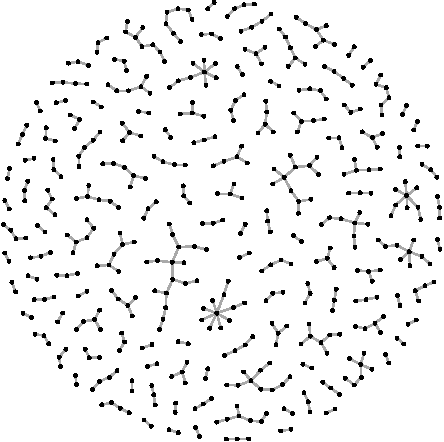
\includegraphics[width=1\linewidth]{paper-blocking_files/figure-latex/dedup_graph-1}

We create a long \texttt{data.table} with information on blocks and units from the original dataset.

\begin{verbatim}
df_block_melted <- melt(result_dedup_hnsw$result, id.vars = c("block", "dist"))
df_block_melted_rec_block <- unique(df_block_melted[, .(rec_id=value, block)])
head(df_block_melted_rec_block)
\end{verbatim}

\begin{verbatim}
#>    rec_id block
#>     <int> <num>
#> 1:      1    35
#> 2:      2     1
#> 3:      3    88
#> 4:      4    13
#> 5:      5     2
#> 6:      6    35
\end{verbatim}

We add the block information to the final dataset.

\begin{verbatim}
RLdata500[df_block_melted_rec_block, on = "rec_id", block_id := i.block]
head(RLdata500)
\end{verbatim}

\begin{verbatim}
#>    fname_c1 fname_c2 lname_c1 lname_c2    by     bm     bd rec_id ent_id
#>      <char>   <char>   <char>   <char> <int> <char> <char>  <int>  <int>
#> 1:  CARSTEN             MEIER           1949     07     22      1     34
#> 2:     GERD             BAUER           1968     07     27      2     51
#> 3:   ROBERT          HARTMANN           1930     04     30      3    115
#> 4:   STEFAN             WOLFF           1957     09     02      4    189
#> 5:     RALF           KRUEGER           1966     01     13      5     72
#> 6:  JUERGEN            FRANKE           1929     07     04      6    142
#>    id_count                    txt block_id
#>       <int>                 <char>    <num>
#> 1:        1   carstenmeier19490722       35
#> 2:        2      gerdbauer19680727        1
#> 3:        1 roberthartmann19300430       88
#> 4:        1    stefanwolff19570902       13
#> 5:        1    ralfkrueger19660113        2
#> 6:        1  juergenfranke19290704       35
\end{verbatim}

We can check in how many blocks the same entities (\texttt{ent\_id}) are observed. In our example, all the same entities are in the same blocks.

\begin{verbatim}
RLdata500[, .(uniq_blocks = uniqueN(block_id)), .(ent_id)][, .N, uniq_blocks]
\end{verbatim}

\begin{verbatim}
#>    uniq_blocks     N
#>          <int> <int>
#> 1:           1   450
\end{verbatim}

Now we can visualize the distances between the units stored in the \texttt{result\_dedup\_hnsw\$result} dataset. Clearly we have a mixture of two groups: matches (close to 0) and non-matches (close to 1).

\begin{verbatim}
hist(result_dedup_hnsw$result$dist, xlab = "Distances", ylab = "Frequency", breaks = "fd",
     main = "Distances calculated between units")
\end{verbatim}

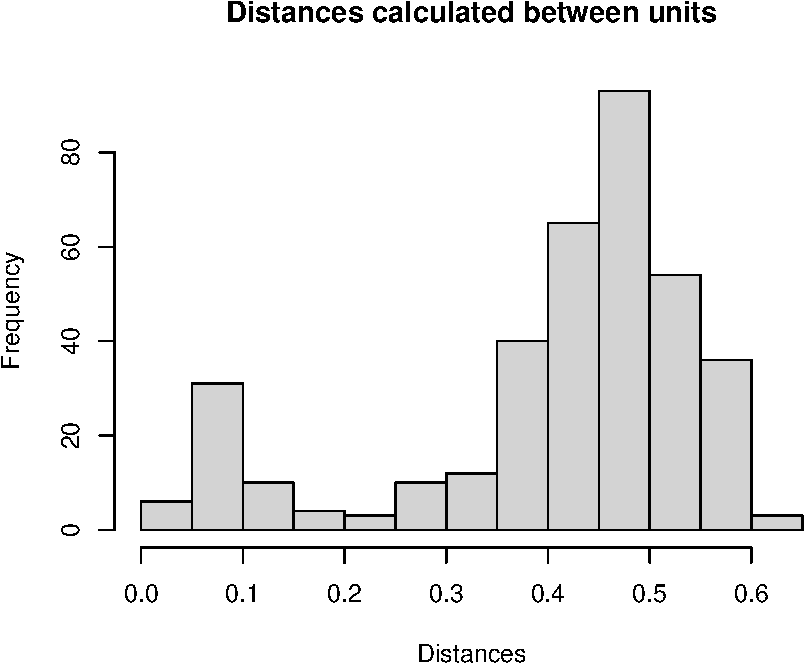
\includegraphics[width=1\linewidth]{paper-blocking_files/figure-latex/dedup_hist-1}

Finally, we visualize the result based on the information whether a block contains matches or not.

\begin{verbatim}
df_for_density <- copy(df_block_melted[block %in% RLdata500$block_id])
df_for_density[, match:= block %in% RLdata500[id_count == 2]$block_id]

plot(density(df_for_density[match==FALSE]$dist), col = "blue", xlim = c(0, 0.8), 
     main = "Distribution of distances between\nclusters type (match=red, non-match=blue)")
lines(density(df_for_density[match==TRUE]$dist), col = "red", xlim = c(0, 0.8))
\end{verbatim}

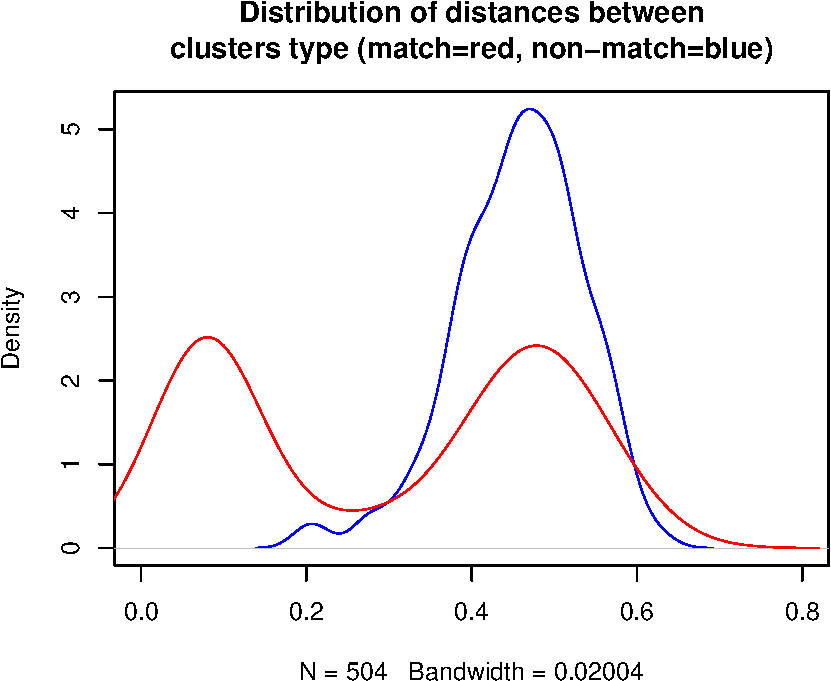
\includegraphics[width=1\linewidth]{paper-blocking_files/figure-latex/dedup_density-1}

Now we compare the evaluation metrics across all ANN algorithms supported by the \texttt{blocking} function, i.e.~NND, HNSW, Approximate Nearest Neighbors Oh Yeah (Annoy, from the \CRANpkg{RcppAnnoy} package), Locality-sensitive hashing (LSH, from the \CRANpkg{mlpack} package), and k-Nearest Neighbors (kNN -- denoted as \texttt{"kd"}, from the \CRANpkg{mlpack} package). We use the \texttt{rec\_id} and \texttt{ent\_id} columns from the \texttt{RLdata500} dataset to specify the true blocks and then calculate evaluation metrics for all algorithms. Additionally, we assess blocking using the \texttt{klsh} function from the \CRANpkg{klsh} package, configured to create 10 blocks and 100 blocks, respectively. In both settings, we use 20 random projections and 2-character shingles. The results are as follows (\texttt{klsh\_10} and \texttt{klsh\_100} refer to the \texttt{klsh} algorithm with 10 blocks and 100 blocks, respectively).

\begin{verbatim}
true_blocks <- RLdata500[, c("rec_id", "ent_id"), with = FALSE]
setnames(true_blocks, old = c("rec_id", "ent_id"), c("x", "block"))
eval_metrics <- list()
ann <- c("nnd", "hnsw", "annoy", "lsh","kd")
for (algorithm in ann) {
  eval_metrics[[algorithm]] <- blocking(x = RLdata500$txt,
                                ann = algorithm,
                                true_blocks = true_blocks)$metrics
}

set.seed(2025)
blocks_klsh_10 <- klsh::klsh(r.set = RLdata500[, c("fname_c1", "fname_c2", "lname_c1",
                                                   "lname_c2", "by", "bm", "bd")],
                             p = 20,
                             num.blocks = 10,
                             k = 2)
klsh_10_metrics <- klsh::confusion.from.blocking(blocking = blocks_klsh_10, 
                                                 true_ids = RLdata500$ent_id)[-1]
klsh_10_metrics$f1_score <- 2 * klsh_10_metrics$precision * klsh_10_metrics$recall / 
  (klsh_10_metrics$precision + klsh_10_metrics$recall)
eval_metrics$klsh_10 <- unlist(klsh_10_metrics)
blocks_klsh_100 <- klsh::klsh(r.set = RLdata500[, c("fname_c1", "fname_c2", "lname_c1",
                                                    "lname_c2", "by", "bm", "bd")],
                              p = 20,
                              num.blocks = 100,
                              k = 2)
klsh_100_metrics <- klsh::confusion.from.blocking(blocking = blocks_klsh_100, 
                                                 true_ids = RLdata500$ent_id)[-1]
klsh_100_metrics$f1_score <- 2 * klsh_100_metrics$precision * klsh_100_metrics$recall /
  (klsh_100_metrics$precision + klsh_100_metrics$recall)
eval_metrics$klsh_100 <- unlist(klsh_100_metrics)

do.call(rbind, eval_metrics) * 100
\end{verbatim}

\begin{verbatim}
#>          recall precision       fpr fnr accuracy specificity f1_score
#> nnd         100 5.0607287 0.7522053   0 99.24810    99.24779 9.633911
#> hnsw        100 4.7573739 0.8027265   0 99.19760    99.19727 9.082652
#> annoy       100 4.8030740 0.7947073   0 99.20561    99.20529 9.165903
#> lsh          98 1.1207685 3.4667201   2 96.53387    96.53328 2.216192
#> kd          100 4.3066322 0.8909383   0 99.10942    99.10906 8.257638
#> klsh_10      82 0.3290794 9.9582999  18 90.03848    90.04170 0.655528
#> klsh_100     86 3.4649476 0.9607057  14 99.03407    99.03929 6.661503
\end{verbatim}

\section{\texorpdfstring{Customizing tooltip design with \pkg{ToOoOlTiPs}}{Customizing tooltip design with }}\label{customizing-tooltip-design-with}

\pkg{ToOoOlTiPs} is a packages for customizing tooltips in interactive graphics, it features these possibilities.

\section{A gallery of tooltips examples}\label{a-gallery-of-tooltips-examples}

The \CRANpkg{palmerpenguins} data \citep{palmerpenguins} features three penguin species which has a lovely illustration by Alison Horst in Figure \ref{fig:penguins-alison}.

\begin{figure}

\includegraphics[width=1\linewidth,height=0.3\textheight,alt={A picture of three different penguins with their species: Chinstrap, Gentoo, and Adelie. }]{figures/penguins} \caption{Artwork by \@allison\_horst}\label{fig:penguins-alison}
\end{figure}

Table \ref{tab:penguins-tab-static} prints at the first few rows of the \texttt{penguins} data:

\begin{table}
\centering
\caption{\label{tab:penguins-tab-static}A basic table}
\centering
\fontsize{7}{9}\selectfont
\begin{tabular}[t]{l|l|r|r|r|r|l|r}
\hline
species & island & bill\_length\_mm & bill\_depth\_mm & flipper\_length\_mm & body\_mass\_g & sex & year\\
\hline
Adelie & Torgersen & 39.1 & 18.7 & 181 & 3750 & male & 2007\\
\hline
Adelie & Torgersen & 39.5 & 17.4 & 186 & 3800 & female & 2007\\
\hline
Adelie & Torgersen & 40.3 & 18.0 & 195 & 3250 & female & 2007\\
\hline
Adelie & Torgersen & NA & NA & NA & NA & NA & 2007\\
\hline
Adelie & Torgersen & 36.7 & 19.3 & 193 & 3450 & female & 2007\\
\hline
Adelie & Torgersen & 39.3 & 20.6 & 190 & 3650 & male & 2007\\
\hline
\end{tabular}
\end{table}

Figure \ref{fig:penguins-ggplot} shows an plot of the penguins data, made using the \CRANpkg{ggplot2} package.

\begin{verbatim}
penguins %>% 
  ggplot(aes(x = bill_depth_mm, y = bill_length_mm, 
             color = species)) + 
  geom_point()
\end{verbatim}

\begin{figure}
\includegraphics[width=1\linewidth]{paper-blocking_files/figure-latex/penguins-ggplot-1} \caption{A basic non-interactive plot made with the ggplot2 package on palmer penguin data. Three species of penguins are plotted with bill depth on the x-axis and bill length on the y-axis. Visit the online article to access the interactive version made with the plotly package.}\label{fig:penguins-ggplot}
\end{figure}

\section{Summary}\label{summary}

We have displayed various tooltips that are available in the package \pkg{ToOoOlTiPs}.

\section{Acknowledgements}\label{acknowledgements}

Work on this package is supported by the National Science Centre, OPUS 20 grant no. 2020/39/B/HS4/00941

\bibliography{RJreferences.bib}

\address{%
Maciej Beręsewicz\\
University of Economics and BusinessStatisical Office in Poznań\\%
Department of Statistics, Poznań, Poland\\ Centre for the Methodology of Population Studies\\
%
\url{https://maciejberesewicz.com}\\%
\textit{ORCiD: \href{https://orcid.org/0000-0002-8281-4301}{0000-0002-8281-4301}}\\%
\href{mailto:maciej.beresewicz@poznan.pl}{\nolinkurl{maciej.beresewicz@poznan.pl}}%
}

\address{%
Adam Struzik\\
Adam Mickiewicz UniversityStatisical Office in Poznań\\%
Department of Mathematics, Poznań, Poland\\ Centre for Urban Statistics\\
%
%
%
\href{mailto:adastr5@st.amu.edu.pl}{\nolinkurl{adastr5@st.amu.edu.pl}}%
}
